\documentclass[12pt,oneside]{book} % for one-sided printing

\usepackage{blindtext}% Just used so we can generate some example text
\usepackage{amsmath}
\usepackage{algorithm}
\usepackage{algpseudocode}
\usepackage{amssymb}
\usepackage{mathtools}
\usepackage[export]{adjustbox}
\usepackage{lipsum}
\usepackage{booktabs}  % For better quality tables
\usepackage{longtable} % Pour les tableaux sur plusieurs pages
\usepackage{tabularx}  % for the X column type
\usepackage{listings}
\usepackage{xcolor}
\usepackage{caption}
\usepackage{xfrac}
\usepackage{indentfirst}
\usepackage{subcaption}
\usepackage{graphicx}
\usepackage{geometry}
\geometry{a4paper, margin=1in}

% Place style file after other packages.
\usepackage{cranfieldthesis}
\usepackage{lscape} % for landscape pages
\usepackage{float}
\usepackage[toc,title,page]{appendix}

% Couleurs personnalisées
\definecolor{backcolour}{rgb}{0.96, 0.96, 0.96} % Fond très clair
\definecolor{codegray}{rgb}{0.47, 0.47, 0.47}   % Commentaires et numéros de ligne
\definecolor{codegreen}{rgb}{0.25, 0.50, 0.35}  % Commentaires
\definecolor{codeblue}{rgb}{0.26, 0.44, 0.58}   % Mots-clés
\definecolor{codepurple}{rgb}{0.50, 0, 0.50}    % Identificateurs
\definecolor{codeteal}{rgb}{0, 0.5, 0.5}        % Chaînes de caractères
\definecolor{terminalback}{rgb}{0.05, 0.05, 0.05} % Fond très sombre pour le terminal
\definecolor{terminaltext}{rgb}{0.7, 0.7, 0.7}    % Texte clair pour le terminal
\definecolor{mygreen}{rgb}{0,0.6,0}
\definecolor{mygray}{rgb}{0.5,0.5,0.5}
\definecolor{mymauve}{rgb}{0.58,0,0.82}
\definecolor{terminalbgcolor}{HTML}{330033}
\definecolor{terminalrulecolor}{HTML}{000099}

\lstdefinestyle{bashstyle}{
    language=bash,
    backgroundcolor=\color{backcolour},
    basicstyle=\ttfamily\scriptsize,
    keywordstyle=\color{blue},
    stringstyle=\color{red},
    identifierstyle=\color{codepurple},
    commentstyle=\color{codegreen},
    morecomment=[l]{\#},   % Define comment style
    frame=single,          % adds a frame around the code
    rulecolor=\color{gray},% if not set, the frame-color may be changed on line-breaks
    breakatwhitespace=false,
    breaklines=true,       % sets automatic line breaking
    captionpos=b,          % sets the caption-position to bottom
    keepspaces=true,       % keeps spaces in text
    showspaces=false,      % show spaces everywhere adding particular underscores
    showstringspaces=false % underline spaces within strings only
}

\lstdefinestyle{cstyle}{
    language=C++,
    basicstyle=\ttfamily\scriptsize,
    keywordstyle=\color{blue},
    backgroundcolor=\color{backcolour},
    stringstyle=\color{red},
    commentstyle=\color{codegreen},
    morecomment=[l][\color{magenta}]{\#},
    breaklines=true,
    numbers=left,
    numberstyle=\tiny\color{gray},
    showstringspaces=false,
    tabsize=2,
    frame=single
}

% Title Page Set Up
\title{Artificial Intelligence Assignment}
\author{Alexis Balayre}
\date{18\textsuperscript{th} March 2024}
\school{\SATM}
\degree{MSc}
\course{Computational Software of Techniques Engineering}
\academicyear{2023 - 2024}

% Supervisors
\supervisor{Dr Jun Li}

% Copyright
\copyrightyear{2024}

% References
\usepackage[numbers]{natbib} % for nice referencing
\makeatletter % Reference list option change to number and period
\renewcommand\@biblabel[1]{#1.} % from [1] to 1
\makeatother %
\setcitestyle{round} % use round citations

\begin{document}

\frontmatter

% Form Title Pages
\maketitle

% Abstract and Keywords
\begin{abstract}

    ru

\end{abstract}

% Use single spacing for Table of Contents, List of Figures, etc
{
\clearpage
\singlespacing
% Table of Contents
{
    \tableofcontents
}
\clearpage

% List of Figures
\listoffigures

% List of Tables
\listoftables
}

%% Main Matter
\mainmatter
\pagestyle{fancy}
\fancyhead[L]{\nouppercase{\leftmark}}
\fancyhead[R]{\nouppercase{\rightmark}}

\chapter{Introduction}
The use of artificial intelligence in the medical field represents a major
development in diagnostics, opening up new avenues for the accurate detection
of disease through the analysis of medical images. This report explores the
impact of AI on improving the interpretation of chest X-rays, a field
characterised by its intrinsic complexity and the crucial need for diagnostic
accuracy for effective patient management. This research project was stimulated
by a challenge from Vingroup's Big Data Institute to develop automated systems
capable of accurately identifying and classifying 14 types of thoracic
abnormality from chest X-ray images.

Chest X-rays are essential in the diagnosis of various pathologies, including
potentially fatal conditions such as COVID-19, tuberculosis, and pneumonia.
However, their interpretation can be difficult, not least because of the
subtlety of the pathological signs and the variability of interpretations among
radiologists. Computer-aided detection and diagnosis (CADe/CADx) systems,
enhanced by AI, offer a solution to these challenges, enabling rapid and
accurate analysis of radiographic images, which could significantly improve
clinical decisions and, consequently, patient outcomes.

The aim of this research was to design a deep learning algorithm exploiting a
comprehensive dataset of 18,000 annotated chest scans provided by the
Institute. This model aims to automatically detect abnormalities in chest
X-rays, demonstrating the potential of AI not only as a viable diagnostic
support tool but also as a means of improving diagnostic accuracy and reducing
diagnosis times. By focusing on the detection and classification of thoracic
abnormalities, this initiative seeks to address the pressing needs of
healthcare professionals, particularly in regions where the lack of experienced
radiologists can compromise the quality of patient care.

The creation and validation of such a model represents a significant advance in
the field of radiology, providing healthcare professionals with a reliable
secondary opinion that could reduce the risk of diagnostic errors and improve
patient care pathways. This document describes the methodologies used to
develop the model, the challenges encountered during its development, and the
potential impact of this technological innovation on improving diagnostic
accuracy worldwide.

\chapter{literature Review}

\section{Deep Learning in Medical Imaging}

Deep learning, a branch of artificial intelligence, is characterised by the use
of deep neural networks to model complex representations and perform
classification and prediction tasks on large quantities of data. In the context
of medical imaging, this represents a rapidly expanding area of research that
promises to revolutionise the way imaging data is analysed and interpreted.

\subsection{Potential of deep learning in medical imaging}

Deep learning has demonstrated its potential to improve diagnostic accuracy,
automate repetitive tasks and identify subtle features in medical images.
Algorithms have been developed for the early detection of diseases, such as
cancer, by analysing mammography or magnetic resonance (MR) images.

One of the main strengths of deep learning is its ability to learn directly
from data, without the need for explicit programming. This allows models to be
adapted to a variety of medical imaging tasks, from segmentation to disease
classification~\cite{LITJENS201760}.

\subsection{Challenges and outlook}

Despite advances, the integration of deep learning into everyday clinical
practice faces challenges, including the need for large amounts of annotated
data, concerns about data privacy and security, and the need for rigorous
validation.

Ongoing research aims to overcome these obstacles and explore new applications,
such as improving image quality and predicting disease
progression~\cite{Shen2017}.

\section{Object Detection Methods}

Object detection is a fundamental task in computer vision that involves
identifying and locating objects of different categories in an image or video.
Unlike image classification, which assigns a label to the entire image, object
detection aims to provide a label and bounding box for each object of interest
in the image.

Object detection generally involves two main tasks: object classification
(knowing what objects are) and object localisation (knowing where objects are).
To be successful, an object detection system must be able to recognise objects
under a variety of conditions, such as different sizes, viewing angles, and
occlusion levels. There are two main types of method: two-stage methods and
single-stage methods. These approaches differ mainly in the way they combine
the proposal of regions of interest and object classification.

\subsection{Two-Step Methods}

\subsubsection{Description}

Two-step methods, such as R-CNN and its variants (Fast R-CNN and Faster R-CNN),
start by generating proposals for regions of interest that could contain
objects. They then use a convolution neural network (CNN) to classify the
objects in each proposed region and refine their bounding boxes.

\subsubsection{Benefits}

\begin{itemize}
    \item \textbf{High precision:}These methods allow detailed analysis of each region, leading to highly accurate object detection.
    \item \textbf{Flexibility:} The separation of tasks allows the integration of advanced CNNs for classification, taking advantage of advances in image classification.
\end{itemize}

\subsubsection{Disadvantages}

\begin{itemize}
    \item \textbf{Processing speed:} Individual processing of each region can be slow, which is a disadvantage for real-time applications.
    \item \textbf{Computational complexity:} Generating and evaluating region proposals increases overall complexity.
\end{itemize}

\subsection{One-Step Methods}

\subsubsection{Description}
One-step methods, such as YOLO (You Only Look Once) and SSD (Single Shot
MultiBox Detector), perform bounding box classification and prediction in a
single pass through the network, greatly simplifying the process.

\subsubsection{Benefits}

\begin{itemize}
    \item \textbf{Speed:} Designed to be fast, they facilitate the detection of objects in real time.
    \item \textbf{Simplicity:} Eliminating region proposals reduces complexity and resource requirements.
\end{itemize}

\subsubsection{Disadvantages}

\begin{itemize}
    \item \textbf{Precision:} These methods may be less accurate for certain types of object, particularly small ones or those in groups.
    \item \textbf{Balance between speed and accuracy:} It is often necessary to fine-tune models to balance these aspects.
\end{itemize}

\section{Using metrics to choose the right model}

The performance of object detection models is primarily gauged using two
critical metrics: Average Precision (AP) and Average Recall (AR). These metrics
offer insights into the accuracy and reliability of the model in detecting and
correctly labelling objects across different scenarios.

\begin{itemize}
    \item \textbf{Average Precision (AP):} Measures the precision of the object detection model across various recall levels. Precision here refers to the proportion of true positive detections over the sum of true positive and false positive detections. AP is often averaged over multiple thresholds of Intersection over Union (IoU) to provide a comprehensive measure of model precision.
    \item \textbf{Average Recall (AR):} Assesses the model's ability to detect all relevant objects within an image. It is calculated as the proportion of true positive detections over the sum of true positives and false negatives. AR can be particularly informative when evaluating models on datasets with dense object placements.
    \item \textbf{Intersection over Union (IoU):} Fundamental metric used in object detection to evaluate the accuracy of the bounding boxes drawn by the model. IoU measures the overlap between the predicted bounding box and the ground truth bounding box, expressed as the ratio of their intersection over their union. A detection is classified as a true positive or false positive based on whether the IoU exceeds a specific threshold.
\end{itemize}

\begin{table}[H]
    \centering
    \caption{Recommended Metrics for Various Object Detection Use Cases~\cite{HuggingFaceObjectDetectionLeaderboard}}
    \label{tab:object_detection_metrics}
    \resizebox{\textwidth}{!}{
        \begin{tabular}{@{}lll@{}}
            \toprule
            \textbf{Use Case}                     & \textbf{Real-world Scenarios}          & \textbf{Recommended Metric} \\ \midrule
            General object detection performance  & Surveillance, sports analysis          & AP                          \\
            Low accuracy requirements             & Augmented reality, gesture recognition & AP@.5                       \\
            High accuracy requirements            & Face detection                         & AP@.75                      \\
            Detecting small objects               & Small artifacts in medical imaging     & AP-S                        \\
            Medium-sized objects detection        & Airport security luggage detection     & AP-M                        \\
            Large-sized objects detection         & Detecting vehicles in parking lots     & AP-L                        \\
            Detecting 1 object per image          & Single object tracking in videos       & AR-1                        \\
            Detecting up to 10 objects per image  & Pedestrian detection in street cameras & AR-10                       \\
            Detecting up to 100 objects per image & Crowd counting                         & AR-100                      \\
            Recall for small objects              & Medical imaging for tiny anomalies     & AR-S                        \\
            Recall for medium-sized objects       & Sports analysis for players            & AR-M                        \\
            Recall for large objects              & Wildlife tracking in wide landscapes   & AR-L                        \\ \bottomrule
        \end{tabular}
    }
\end{table}

\chapter{Methodology}

\section{Data Exploration}

\subsection{Overview of the Dataset}

The dataset provided in the VinBigData Chest X-ray Abnormalities Detection
competition consists of 18,000 postero-anterior chest X-ray scans, meticulously
annotated for the presence of various thoracic abnormalities. Each image is
labeled with one or more of 14 distinct abnormality classes, with a dedicated
class for normal observations without findings. The images are stored in DICOM
format, which not only captures the radiographic image but also houses rich
metadata that could potentially enhance analysis and model training.

\subsection{Labeling and Annotations}

Annotations in this dataset are provided by a panel of experienced
radiologists, indicating the presence of 14 critical radiographic findings,
each associated with a bounding box to localize abnormalities within the scans. 

\subsection{Classes and Findings}

The dataset categorizes thoracic abnormalities into 14 classes, with an
additional 15th class for scans without findings:

\begin{table}
    \centering
    \begin{tabular}{|c|c|}
        \hline
        \textbf{Class ID} & \textbf{Name}      \\
        \hline
        0                 & Aortic Enlargement \\
        1                 & Atelectasis        \\
        2                 & Calcification      \\
        3                 & Cardiomegaly       \\
        4                 & Consolidation      \\
        5                 & ILD                \\
        6                 & Infiltration       \\
        7                 & Lung Opacity       \\
        8                 & Nodule/Mass        \\
        9                 & Other Lesion       \\
        10                & Pleural Effusion   \\
        11                & Pleural Thickening \\
        12                & Pneumothorax       \\
        13                & Pulmonary Fibrosis \\
        14                & No Finding         \\
        \hline
    \end{tabular}
    \caption{Classes and associated findings Abnormalities Detection dataset}
    \label{tab:classes}
\end{table}

\subsection{Annotation Distribution Across Classes}
Initial examination of the dataset revealed a notable class imbalance. The
number of annotations per class was visualized in a bar chart (Figure
\ref{fig:annotations_per_class}), showing that certain conditions such as
Aortic Enlargement (Class 0) are more commonly annotated compared to others.
The class 'No finding' (Class 14) had the most annotations, indicating a large
proportion of normal cases.

\begin{figure}[H]
    \centering
    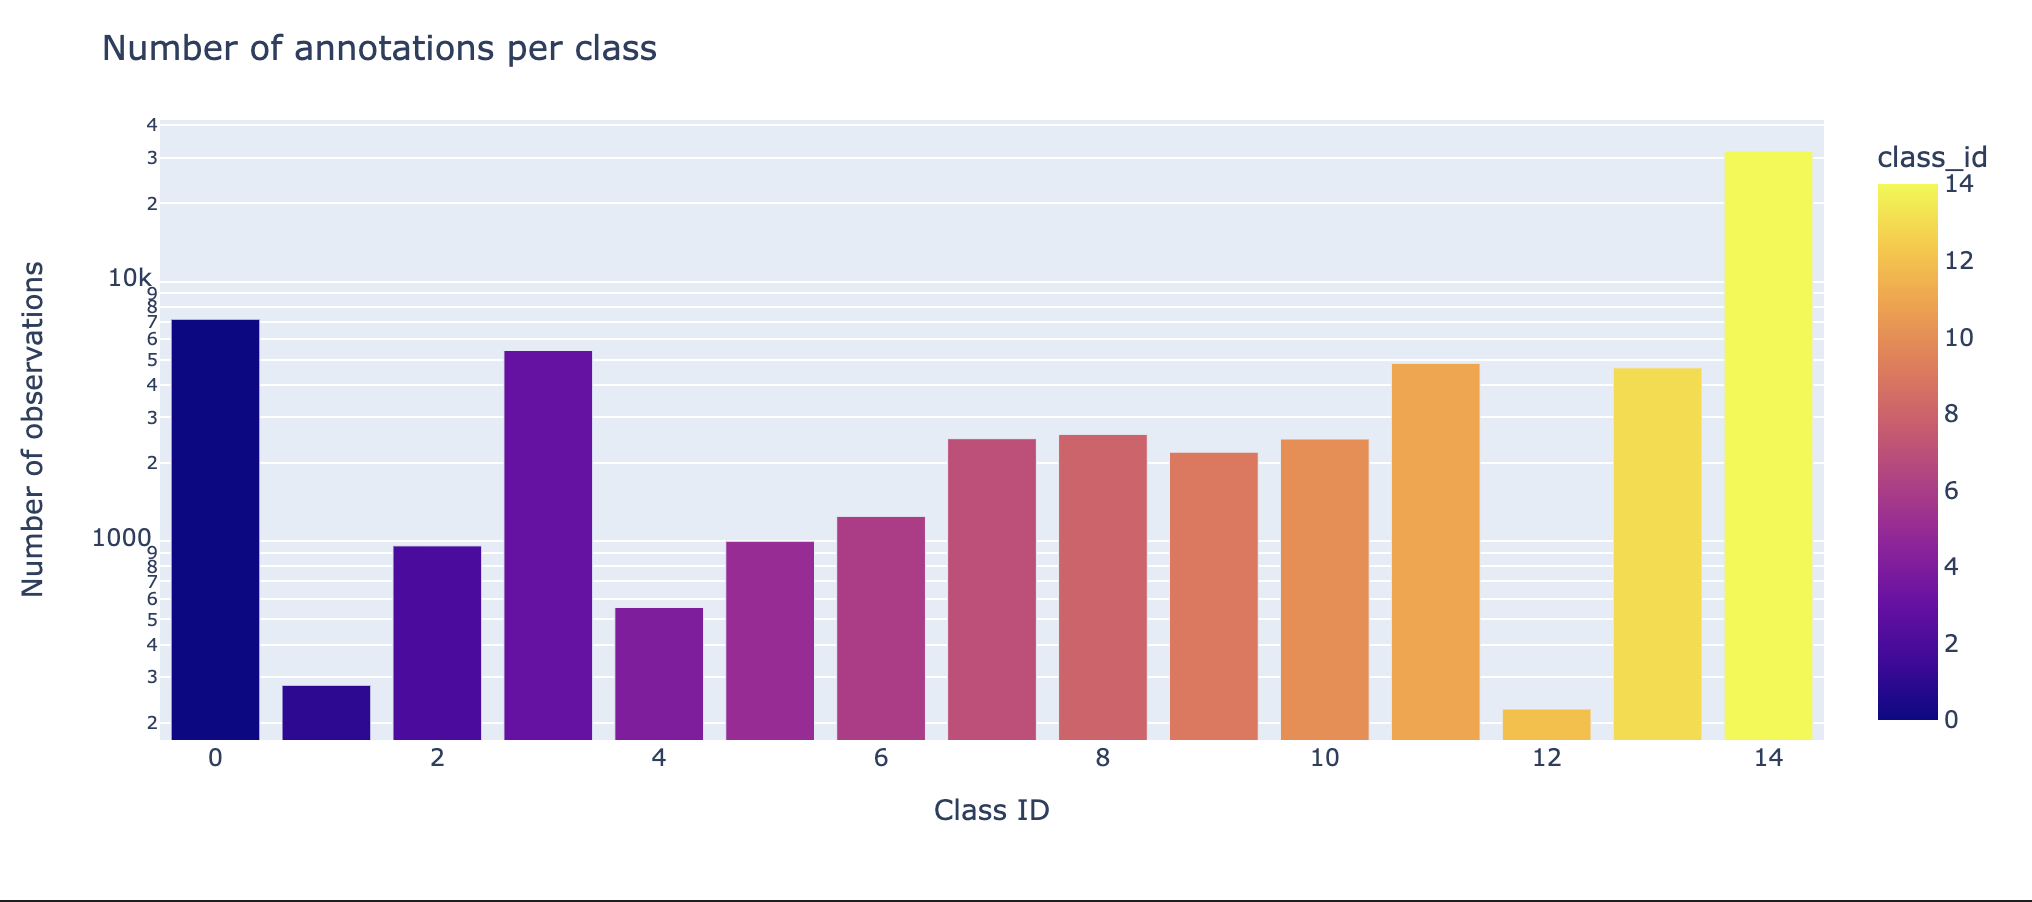
\includegraphics[width=0.8\textwidth]{../results/annotations_per_class.png}
    \caption{Number of annotations per class. The y-axis is on a logarithmic scale to account for the wide range of annotation counts.}
    \label{fig:annotations_per_class}
\end{figure}

\subsection{Annotation Distribution Across Radiologists}
The dataset annotations are also characterized by variability across
radiologists. A bar chart (Figure \ref{fig:annotations_per_rad}) highlights the
number of annotations contributed by each radiologist, with some radiologists
annotating more extensively than others.

\begin{figure}[H]
    \centering
    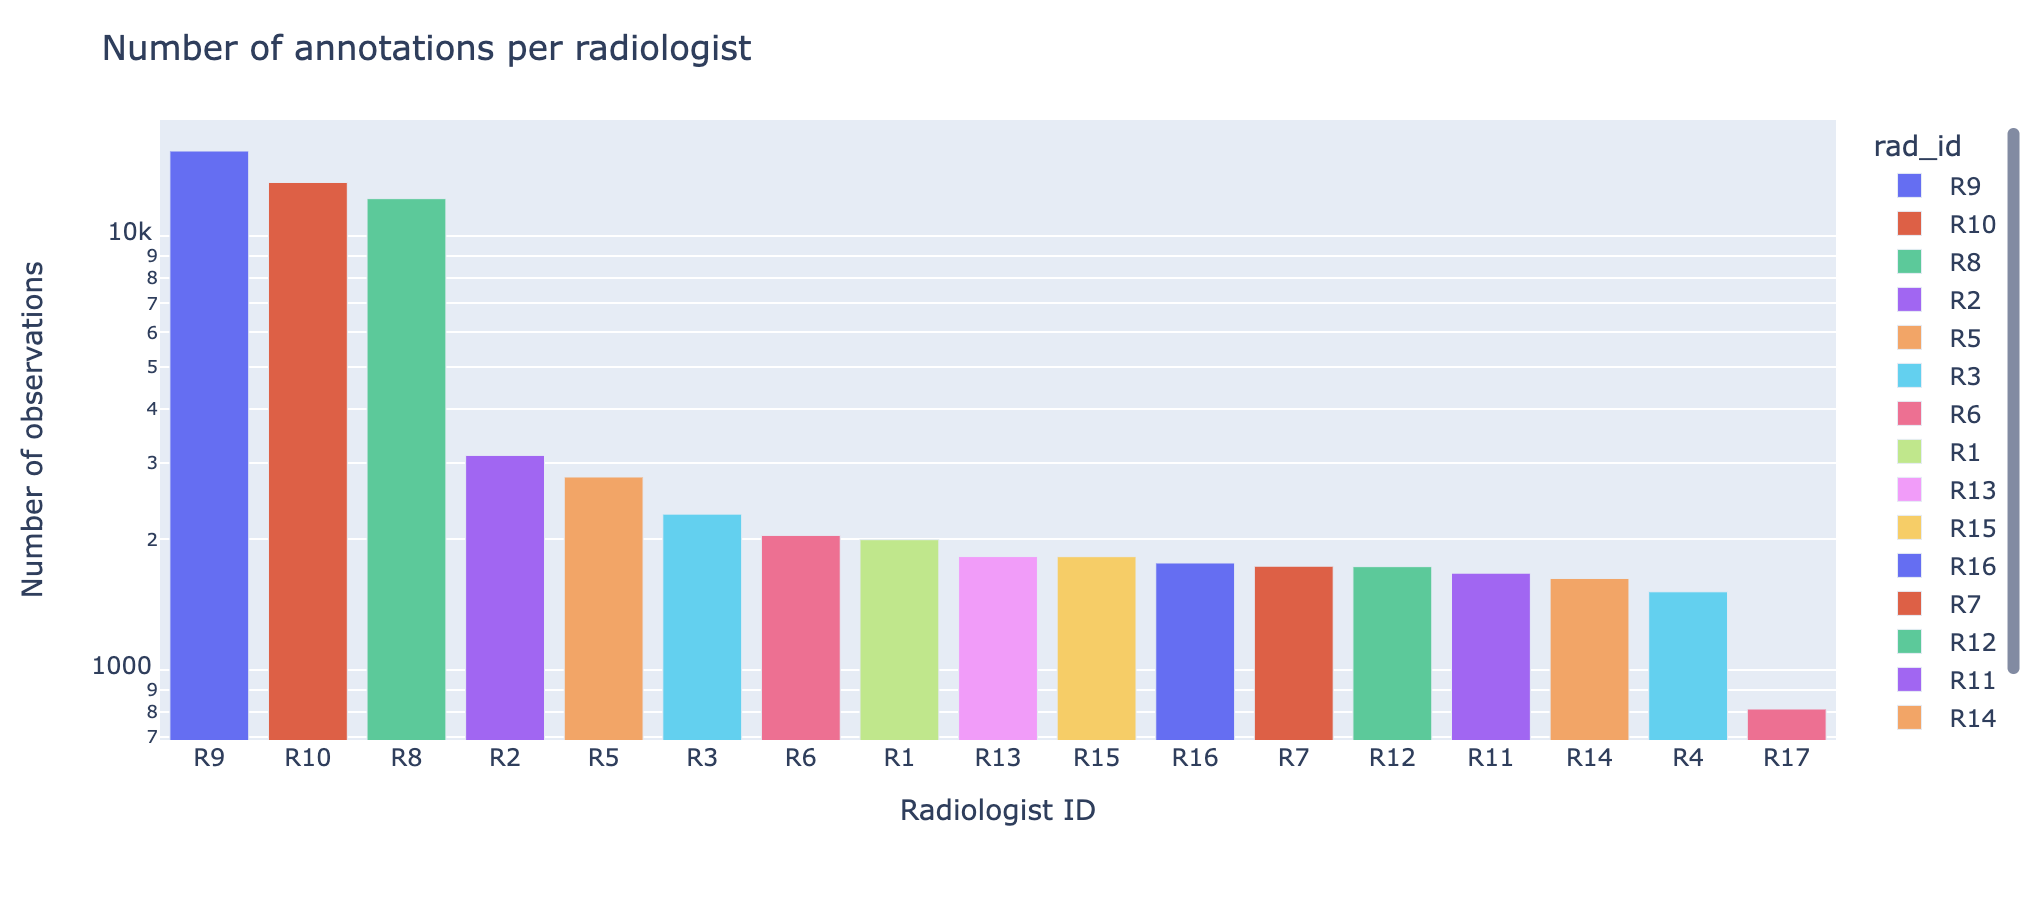
\includegraphics[width=0.8\textwidth]{../results/annotations_per_rad.png}
    \caption{Number of annotations per radiologist. The distribution shows significant variability in the number of annotations made by different radiologists.}
    \label{fig:annotations_per_rad}
\end{figure}

\subsection{Inter-observer Variability}

To further explore the inter-observer variability, a heatmap was constructed
(Figure \ref{fig:annotations_per_rad_class}), showing the interplay between
radiologist IDs and class annotations. This visualization underscored the 'No
finding' class's dominance and revealed discrepancies in the frequency of
annotations per class by different radiologists, suggesting differences in
diagnostic criteria or individual radiologist experience.

\begin{figure}[H]
    \centering
    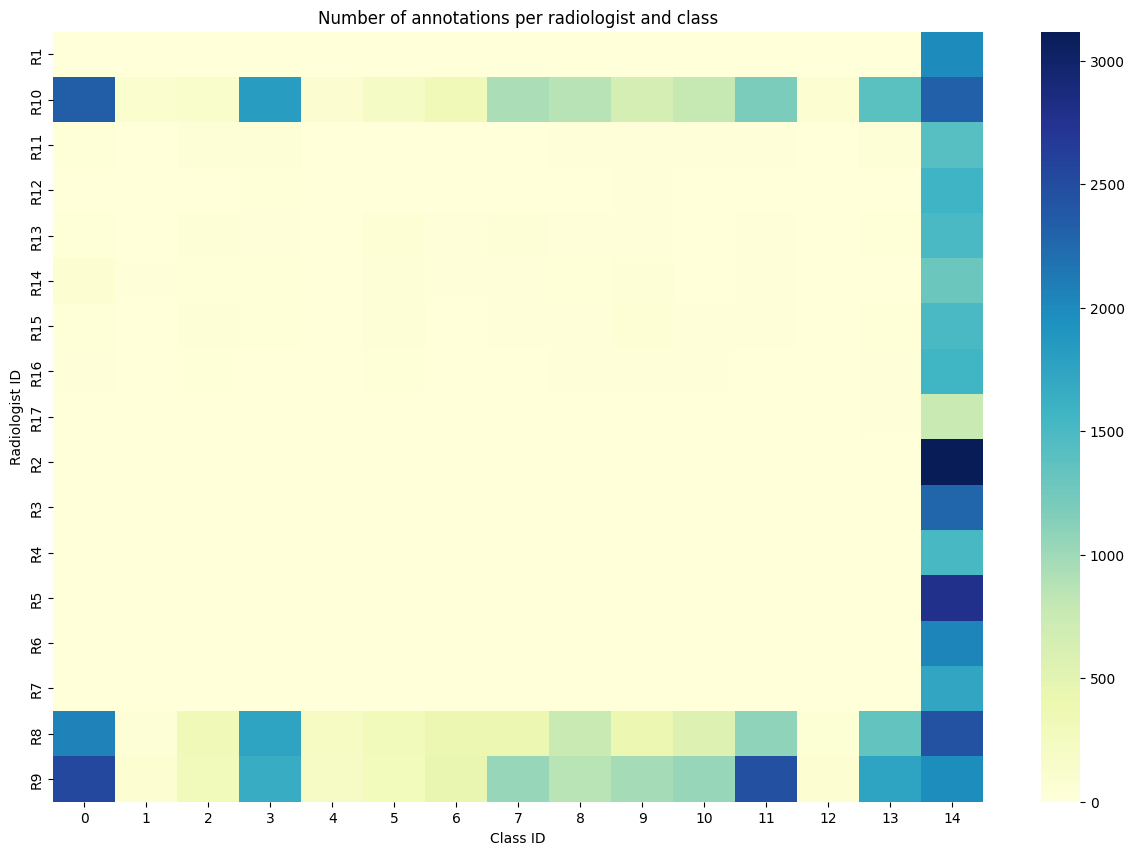
\includegraphics[width=0.8\textwidth]{../results/annotations_per_rad_class.png}
    \caption{Number of annotations per radiologist and class. Darker colors indicate a higher number of annotations, showing a strong prevalence of 'No finding' annotations across all radiologists.}
    \label{fig:annotations_per_rad_class}
\end{figure}

\subsection{Conclusion}
The initial data exploration indicates a rich and complex dataset that presents
certain challenges for machine learning tasks, including class imbalance and
significant inter-observer variability. These insights set the stage for
careful preprocessing, the necessity of balancing techniques, and the
development of sophisticated models that can account for the nuances in
annotation patterns.

\section{Data Extraction and Preprocessing}

The workflow for preparing DICOM files for analysis encompasses three primary
stages, each essential for transforming raw medical images into structured data
amenable to analysis or machine learning applications. These stages are
outlined as follows:

\begin{enumerate}
    \item \textbf{DICOM File Metadata Extraction:}

          The process begins with the extraction of metadata from DICOM files, which are
          rich in information such as patient demographics, study specifics, and imaging
          parameters. This extraction is facilitated by the \texttt{pydicom} library,
          enabling the reading of each DICOM file and the retrieval of pertinent metadata
          fields. The collected metadata is subsequently stored in a CSV file, offering
          straightforward access and the ease of subsequent analysis.

    \item \textbf{DICOM File Pixel Array Processing and Extraction:}

          Following metadata extraction, attention turns to the DICOM files' pixel data.
          This phase includes applying the Value of Interest (VOI) Look-Up Table (LUT)
          for image normalization, adjusting images based on their photometric
          interpretation (e.g., inverting "MONOCHROME1" images), and scaling the pixel
          values to an 8-bit format. The processed pixel data is stored in an HDF5 file,
          chosen for its efficiency in managing sizable datasets and facilitating fast
          access to individual images.

    \item \textbf{DICOM File Features Extraction:}

          The concluding stage involves extracting salient features from the processed
          images. This encompasses computing features related to texture, shape, and
          intensity histograms to quantitatively describe each image's essential
          characteristics. These features are vital for training machine learning models,
          as they provide a numeric representation of the images. The extracted features
          are assembled into a structured dataset, usually saved in a CSV file, ready for
          in-depth analysis or model training.
\end{enumerate}

This enumerated workflow systematically transforms DICOM files into a
structured format, setting the stage for comprehensive medical image analysis
and the development of predictive models.

section{Faster R-CNN Model}

The Faster R-CNN model is a deep learning architecture for object detection,
consisting of two main components: a Region Proposal Network (RPN) and a Fast
R-CNN object detection network. The workflow of this model can be described as
follows:

\subsection{Region Proposal Network (RPN)}

The RPN is a fully convolutional network that operates on the feature maps
$\mathbf{X}$ generated by the backbone network (e.g., ResNet-50). It generates
object proposals by classifying anchor boxes $\mathbf{a}$ as either containing
an object or not, and also refines the bounding box coordinates for positive
proposals.

The RPN outputs a set of object proposals $\mathbf{R} = \{\mathbf{r}_1,
    \mathbf{r}_2, \ldots, \mathbf{r}_n\}$, where each proposal $\mathbf{r}_i =
    (p_i, b_i)$ consists of a probability score $p_i$ indicating the likelihood of
containing an object, and a bounding box $b_i$ represented by its coordinates.

The RPN is trained using a multi-task loss function:

\begin{equation}
    L_{\text{RPN}} = \frac{1}{N_{\text{cls}}} \sum_{i} L_{\text{cls}}(p_i, p_i^*) + \lambda \frac{1}{N_{\text{reg}}} \sum_{i} p_i^* L_{\text{reg}}(b_i, b_i^*)
\end{equation}

where $L_{\text{cls}}$ is the classification loss (e.g., cross-entropy loss),
$L_{\text{reg}}$ is the bounding box regression loss (e.g., smooth L1 loss),
$p_i^*$ and $b_i^*$ are the ground truth labels for proposal $i$,
$N_{\text{cls}}$ and $N_{\text{reg}}$ are normalization factors, and $\lambda$
is a balancing weight.

\subsection{Fast R-CNN Network}

The Fast R-CNN network is responsible for classifying the proposed RoIs and
refining their bounding box coordinates. It takes the feature maps $\mathbf{X}$
from the backbone network and the proposed RoIs $\mathbf{R}$ from the RPN as
input.

The RoI pooling layer extracts a fixed-size feature map $\mathbf{x}_i$ from
each RoI $\mathbf{r}_i$, which is then fed into fully connected layers for
classification and bounding box regression:

\begin{equation}
    p_{\text{cls}}(c | \mathbf{x}_i) = \text{Softmax}(W_{\text{cls}}^T \mathbf{x}_i + b_{\text{cls}})
\end{equation}
\begin{equation}
    b_{\text{reg}}(\mathbf{x}_i) = W_{\text{reg}}^T \mathbf{x}_i + b_{\text{reg}}
\end{equation}

where $p_{\text{cls}}(c | \mathbf{x}_i)$ is the predicted probability of RoI
$\mathbf{x}_i$ belonging to class $c$, and $b_{\text{reg}}(\mathbf{x}_i)$ is
the predicted bounding box regression offsets for $\mathbf{x}_i$.
$W_{\text{cls}}$, $W_{\text{reg}}$, $b_{\text{cls}}$, and $b_{\text{reg}}$ are
learnable parameters.

The Fast R-CNN network is trained using a multi-task loss function similar to
the RPN:

\begin{equation}
    L_{\text{Fast R-CNN}} = \frac{1}{N_{\text{cls}}} \sum_{i} L_{\text{cls}}(p_{\text{cls}}(c | \mathbf{x}_i), c_i^*) + \lambda \frac{1}{N_{\text{reg}}} \sum_{i} c_i^* L_{\text{reg}}(b_{\text{reg}}(\mathbf{x}_i), b_i^*)
\end{equation}

where $c_i^*$ and $b_i^*$ are the ground truth labels for RoI $\mathbf{x}_i$,
and $\lambda$ is a balancing weight.

\subsection{Model Training and Evaluation}

The overall loss function for the Faster R-CNN model is the sum of the RPN loss
and the Fast R-CNN loss:

\begin{equation}
    L = L_{\text{RPN}} + L_{\text{Fast R-CNN}}
\end{equation}

The model is trained by minimizing this loss function using an optimization
algorithm, such as Stochastic Gradient Descent (SGD) with momentum and weight
decay.

During evaluation, the model's performance is assessed using metrics such as
mean Average Precision (mAP) and mean Average Recall (mAR). These metrics
measure the average precision and recall across different classes and
confidence thresholds, providing an overall performance score for object
detection.

\section{Model Overview}
Our model is an implementation of Faster R-CNN, leveraging a ResNet-50 backbone
for the task of detecting thoracic abnormalities in chest X-ray images. The
Faster R-CNN framework combines a Region Proposal Network (RPN) with a Fast
R-CNN detector to efficiently identify and localize abnormalities.

\subsection{Mathematical Foundation}
\subsubsection{Region Proposal Network (RPN)}
The RPN generates region proposals using a sliding window over the
convolutional feature map obtained from the backbone. For each location, it
predicts multiple potential bounding boxes and objectness scores. This can be
formalized as:

\begin{equation}
    O, B = \text{RPN}(F)
\end{equation}

where $F$ represents the feature map, $O$ the objectness score, and $B$ the
bounding box coordinates for each proposal.

\subsubsection{Anchor Boxes}
Anchor boxes are predefined boxes of various scales and aspect ratios that
serve as references at each sliding position. The RPN adjusts these anchors to
better fit the objects. The adjustment is a regression problem, typically using
a smooth L1 loss:

\begin{equation}
    L_{\text{reg}} = \text{smooth}_{L1}(B_{\text{pred}}, B_{\text{gt}})
\end{equation}

where $B_{\text{pred}}$ are the predicted box adjustments and $B_{\text{gt}}$
the ground truth box adjustments.

\subsubsection{Fast R-CNN Detector}
The Fast R-CNN detector uses the proposals from the RPN, applying RoI Pooling
to extract a fixed-size feature vector for each. These are then passed through
fully connected layers to classify the object and refine the bounding box:

\begin{equation}
    C, B' = \text{Fast R-CNN}(F_{\text{roi}})
\end{equation}

where $F_{\text{roi}}$ are the RoI-pooled features, $C$ the class predictions,
and $B'$ the refined bounding box predictions.

\subsection{Training Workflow}
\subsubsection{Loss Functions}
The total loss for training the Faster R-CNN model is a combination of the RPN
loss and Fast R-CNN loss:

\begin{equation}
    L = L_{\text{cls}}^{\text{RPN}} + L_{\text{reg}}^{\text{RPN}} + L_{\text{cls}}^{\text{Fast R-CNN}} + L_{\text{reg}}^{\text{Fast R-CNN}}
\end{equation}

where $L_{\text{cls}}$ and $L_{\text{reg}}$ denote the classification and
regression losses, respectively, for each component.

\subsubsection{Multi-Task Training}
The model is trained end-to-end with a multi-task loss that optimizes both the
RPN and Fast R-CNN simultaneously. This approach efficiently shares the
convolutional features between the RPN and detector, significantly reducing the
computational cost compared to training separate models.

\subsection{Evaluation Metrics}
Model performance is assessed using mean Average Precision (mAP) and mean
Average Recall (mAR) across different Intersection over Union (IoU) thresholds,
providing a comprehensive evaluation of detection accuracy.

\subsubsection{Mean Average Precision (mAP)}
The mAP is calculated by averaging the precision across different recall levels
for each class and then averaging over all classes:

\begin{equation}
    \text{mAP} = \frac{1}{|C|} \sum_{c \in C} \text{AP}_c
\end{equation}

where $C$ is the set of classes and $\text{AP}_c$ the average precision for
class $c$.

\subsubsection{Mean Average Recall (mAR)}
Similarly, mAR measures the average recall across different precision levels,
providing insight into the model's ability to detect all relevant instances.

\section{Evaluation metrics for Faster R-CNN}

To evaluate the performance of the Faster R-CNN model in the object detection
task task, several metrics are used. These metrics provide a quantitative
measure of the model's ability to correctly identify and locate objects in
images.

\subsection{Intersection over Union (IoU)}

Intersection over Union (IoU) is a key metric for assessing the accuracy of of
the bounding boxes predicted by the model. It is defined as the ratio between
the area of the intersection and the area of the union of the predicted and
ground truth:

\begin{equation}
    IoU = \frac{\text{Intersection area}}{\text{Union area}}
\end{equation}

A prediction is considered correct if the IoU with a ground truth box field
exceeds a certain threshold, typically set at 0.5.

\subsection{Precision and Recall}

Precision is the proportion of positive identifications that are correct, while
recall is the proportion of actual ground truths that are truths that are
correctly identified. They are calculated as follows:

\begin{equation}
    \text{Precision} = \frac{TP}{TP + FP}
\end{equation}

\begin{equation}
    \text{Recall} = \frac{TP}{TP + FN}
\end{equation}

where $TP$ represents true positives, $FP$ false positives, and $FN$ false
negatives.

\subsection{Mean Average Precision (mAP)}

The mean Average Precision (mAP) is the average of the APs calculated for each
class of objects over different IoU thresholds. The AP for a class is the area
under the precision-recall curve, and the mAP is an average of these values for
all classes:

\begin{equation}
    mAP = \frac{1}{N} \sum_{i=1}^{N} AP_i
\end{equation}

where $N$ is the number of classes and $AP_i$ is the Average Precision for
class $i$.

These metrics provide a comprehensive assessment of the performance of the
Faster R-CNN model, measuring how accurately the model is able to detect and
locate objects in different images.

\chapter{Results and Discussion}
\section{Results}

\begin{figure}[H]
    \centering
    \begin{minipage}[b]{0.45\textwidth}
        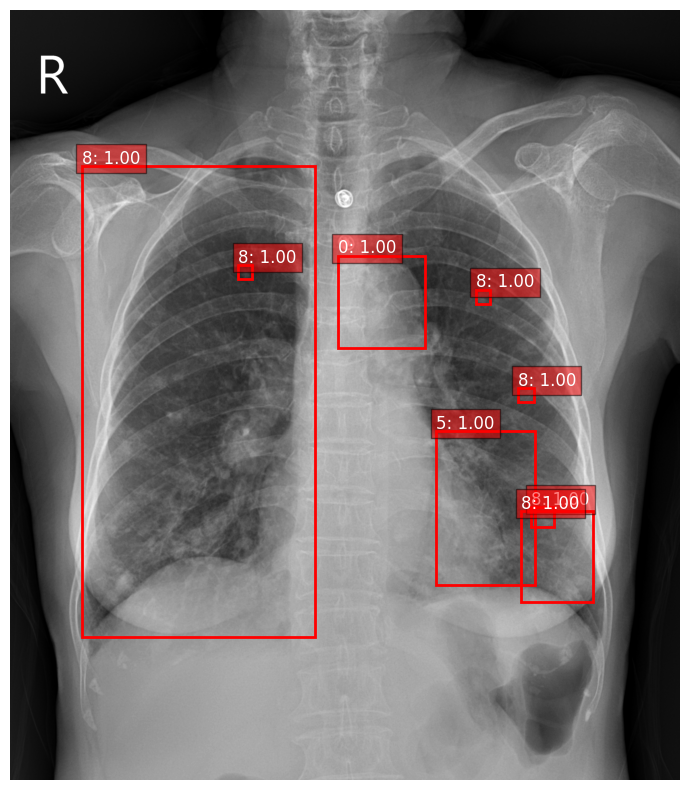
\includegraphics[width=\textwidth]{../results/true_labels.png}
        \caption{True Labels}
        \label{fig:true_labels}
    \end{minipage}
    \hfill % This inserts a space between the images. Adjust the space as needed.
    \begin{minipage}[b]{0.45\textwidth}
        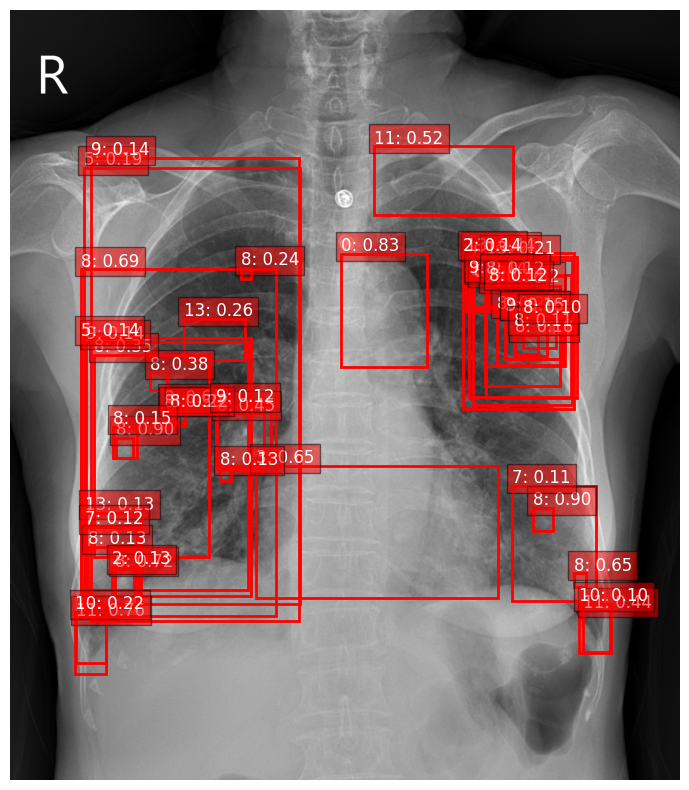
\includegraphics[width=\textwidth]{../results/predictions.png}
        \caption{Predicted labels}
        \label{fig:predictions_without_filter} % Make sure the label matches the description
    \end{minipage}
\end{figure}

\begin{figure}[H]
    \centering
    \begin{minipage}[b]{0.45\textwidth}
        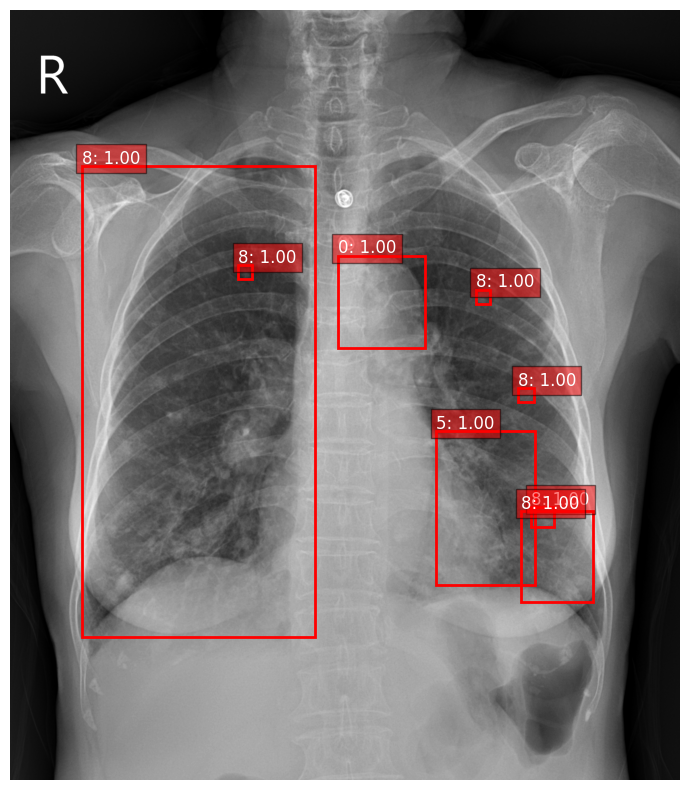
\includegraphics[width=\textwidth]{../results/true_labels.png}
        \caption{True Labels}
        \label{fig:true_labels}
    \end{minipage}
    \hfill % This inserts a space between the images. Adjust the space as needed.
    \begin{minipage}[b]{0.45\textwidth}
        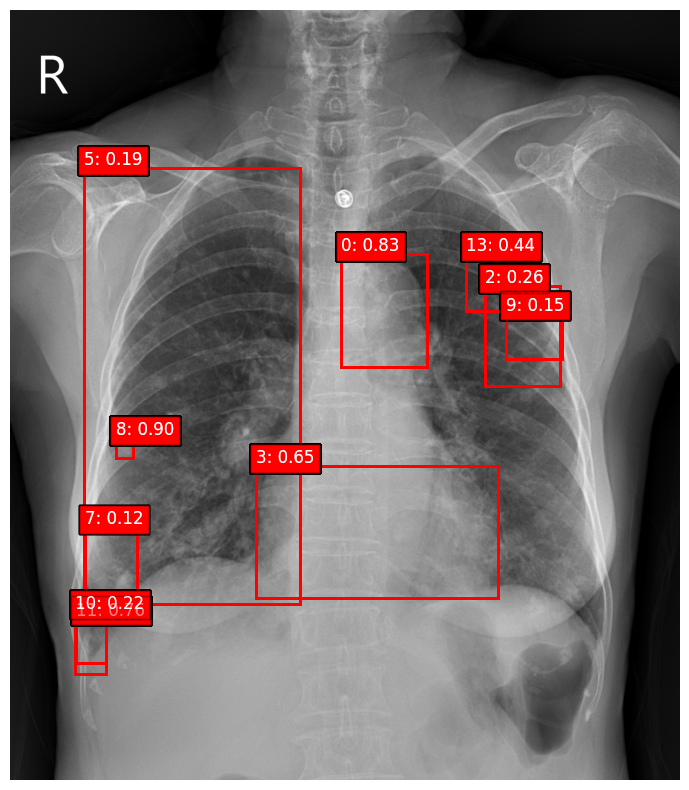
\includegraphics[width=\textwidth]{../results/predictions_with_filter.png}
        \caption{Filtered Predicted labels}
        \label{fig:predictions_with_filter} % Make sure the label matches the description
    \end{minipage}
\end{figure}


\begin{table}[H]
    \centering
    \begin{tabular}{|c|c|c|c|c|c|c|c|c|}
        \hline
        \textbf{Class} & \textbf{TP} & \textbf{FP} & \textbf{FN} & \textbf{Precision} & \textbf{Recall} & \textbf{F1 Score} & \textbf{mAP} & \textbf{mAR@100} \\ \hline
        0              & 1031        & 1810        & 219         & 0.363              & 0.825           & 0.504             & 0.3933       & 0.7924           \\ \hline
        1              & 24          & 156         & 25          & 0.133              & 0.490           & 0.210             & 0.0555       & 0.3333           \\ \hline
        2              & 64          & 806         & 94          & 0.074              & 0.405           & 0.125             & 0.0252       & 0.3472           \\ \hline
        3              & 694         & 1802        & 159         & 0.278              & 0.814           & 0.414             & 0.4062       & 0.8071           \\ \hline
        4              & 45          & 485         & 48          & 0.085              & 0.484           & 0.144             & 0.0424       & 0.3614           \\ \hline
        5              & 139         & 1080        & 66          & 0.114              & 0.678           & 0.195             & 0.0906       & 0.5267           \\ \hline
        6              & 178         & 1512        & 70          & 0.105              & 0.718           & 0.184             & 0.1054       & 0.6096           \\ \hline
        7              & 454         & 4786        & 143         & 0.087              & 0.760           & 0.156             & 0.0661       & 0.5791           \\ \hline
        8              & 268         & 2544        & 166         & 0.095              & 0.618           & 0.165             & 0.1339       & 0.5633           \\ \hline
        9              & 215         & 2800        & 205         & 0.071              & 0.512           & 0.125             & 0.0539       & 0.3444           \\ \hline
        10             & 498         & 2431        & 101         & 0.170              & 0.831           & 0.282             & 0.2124       & 0.6935           \\ \hline
        11             & 912         & 10079       & 269         & 0.083              & 0.772           & 0.150             & 0.0646       & 0.5868           \\ \hline
        12             & 55          & 885         & 9           & 0.059              & 0.859           & 0.110             & 0.3272       & 0.7353           \\ \hline
        13             & 792         & 4841        & 312         & 0.141              & 0.717           & 0.235             & 0.0971       & 0.5115           \\ \hline
        14             & 3799        & 345         & 974         & 0.917              & 0.796           & 0.852             & 0.7276       & 0.7959           \\ \hline
    \end{tabular}
    \caption{Extended Evaluation Metrics per Class}
    \label{tab:extended_metrics}
\end{table}

\section{AI Ethical challenges in the medical sector}

While the use of artificial intelligence in radiology holds enormous
transformative potential for the medical sector, this application nevertheless
raises a number of significant ethical issues and challenges, requiring careful
thought and innovative solutions to ensure that the development and use of AI
in medicine is done in an ethical and responsible manner.

\subsection{Respect for Confidentiality and Data Security}

The first ethical challenge concerns the confidentiality and security of
patient data. AI systems, such as those developed to detect thoracic anomalies
from X-rays, require access to large volumes of sensitive medical data. It is
imperative to ensure that this data is protected from unauthorised access or
misuse, in compliance with regulations such as the RGPD in Europe or HIPAA in
the United States. The implementation of advanced cryptographic techniques and
access management systems is essential to secure this information.

\subsection{Algorithmic bias and fairness}

Another major issue is the risk of algorithmic bias, which can lead to unfair
diagnoses. The datasets used to train AI systems may reflect existing biases,
resulting in variable performance across demographic groups. This raises the
issue of fairness in automated diagnoses, where certain populations could be
disadvantaged. To counter this problem, it is crucial to ensure that datasets
are diverse and representative, and to develop methodologies for identifying
and correcting algorithmic biases.

\section{Transparency and Explicability}

The transparency and explicability of decisions made by AI systems is a central
ethical challenge. The decision-making mechanisms of complex AI models, such as
deep neural networks, are often perceived as a "black box", making it difficult
to understand and justify the diagnoses proposed. It is therefore imperative to
work towards more explainable AI models, enabling healthcare professionals to
understand and validate the recommendations provided by these systems before
making clinical decisions.

\section{Responsibility and Professional Autonomy}

The question of liability in the event of diagnostic errors involving AI is
also a cause for concern. Determining the share of responsibility between the
creators of AI systems, the healthcare professionals using them, and healthcare
institutions requires in-depth legal and ethical reflection. Furthermore, the
use of AI should not erode the professional autonomy of radiologists, but
rather serve as a complementary tool enabling them to improve their accuracy
and efficiency.

\subsection{Conclusion}

While AI promises to revolutionise the field of radiology, ensuring faster and
more accurate diagnoses, it is essential to tackle the ethical challenges it
raises head on.This requires close collaboration between AI developers,
healthcare professionals, regulators, and patients, to ensure that these
technologies advance in an ethical manner, enhancing the quality of medical
care while respecting patients' rights and dignity.

\chapter{Conclusion}

\bibliographystyle{CranfieldNumbered}
\bibliography{CUCitations}

%TC:ignore 
\appendix
\chapter{Source Codes}
\begin{subappendices}
    \section{Dataset Class}\label{appendix:ChestXrayDataset}
    \lstinputlisting[style=cstyle]{../Faster-R-CNN/ChestXrayDataset.py}

    \newpage
    \section{Data Module Class}\label{appendix:ChestXrayDataModule}
    \lstinputlisting[style=cstyle]{../Faster-R-CNN/ChestXrayDataModule.py}

    \newpage
    \section{Faster-R-CNN Lightning Model Class}\label{appendix:ChestXrayLightningModel}
    \lstinputlisting[style=cstyle]{../Faster-R-CNN/ChestXrayLightningModel.py}
\end{subappendices}

%TC:endignore 

\end{document}

